\chapter{La postura e ciò che la influenza}

La posturologia studia l’essere umano nel suo ambiente vitale ed è la prima a servirsi dei riflessi posturali per l’analisi di patologie funzionali. La postura è definita come “il modo di stare in equilibrio nelle varie posizioni”, ed esprime una funzione relativa ai modi e alle capacità del corpo umano di acquisire e mantenere tutte le posizioni, conservando l’equilibrio. 

Il sistema dell’equilibrio può essere considerato un sistema complesso e aperto: complesso perché costituito da un insieme di sottoinsiemi reciprocamente interrelazionati, aperto perché ciascuno di essi interagisce con l’ambiente e con la situazione in atto. Ogni componente del sistema è in rapporto con tutte le altre parti che lo costituiscono e va incontro a modificazioni, conseguentemente alle variazioni di queste ultime, al fine di costruire un insieme funzionale stabile. 

Il sistema che regola la staticità del corpo nello spazio è il sistema tonico posturale. Il Sistema-Tonico-Posturale (STP) è un sistema cibernetico, un circuito che necessita di un’afferenza (input), proveniente dagli esterocettori e propriocettori, di centri superiori di modulazione, integrazione, pianificazione, risposta, controllo e di un’efferenza (output) che traduce il segnale elaborato dai centri superiori in gesto motorio (Schema in Figura 2.1). Il suo studio consente di discriminare al meglio fra gli elementi determinanti la causa primaria di una sindrome patologica. 
\\\ \\\ \\\ \\\ \\\ \\\ \\\
Le strutture recettoriali concorrono nell’apportare informazioni posturali, che, una volta elaborate, migliorano l’equilibrio muscolare. Queste sono:

 \begin{itemize}
 \itemsep-0.6em 
 \item[--]occhio: la formazione dell’immagine retinica fornisce all’individuo informazioni relative ai suoi movimenti nello spazio. I recettori visivi sono i coni e i bastoncelli che informano sulla situazione ambientale
 \item[--]apparato stomatognatico
 \item[--]sistema vestibolare: endolinfa e otoliti dell’orecchio interno determinano importanti adeguamenti del sistema posturale in relazione alle tre dimensioni dello spazio, da coordinare/integrare con le informazioni provenienti dagli apparati descritti precedentemente
 \item[--]recettori presenti sulla cute della pianta del piede
 \end{itemize}
 
 Il sistema posturale funziona come un insieme che ha lo scopo di lottare contro la forza di gravità per mantenere la posizione eretta equilibrando e coordinando le funzioni a seconda del fine. Ciascun recettore apporta le proprie specifiche informazioni che poi, rielaborate e integrate, daranno luogo allo schema posturale finale. Per realizzare queste funzioni neurofisiologiche, l’organismo utilizza informazioni provenienti sia dall’esterno (esterocettori: sensibili al tocco, alla pressione e al movimento) che dall’interno (enterocettori, propriocettori: danno informazioni sulle risposte statiche e dinamiche dei muscoli e sulle tensioni esercitate sui tendini).
 \\\ \\\
 \begin{figure}[h!]
	\centering
	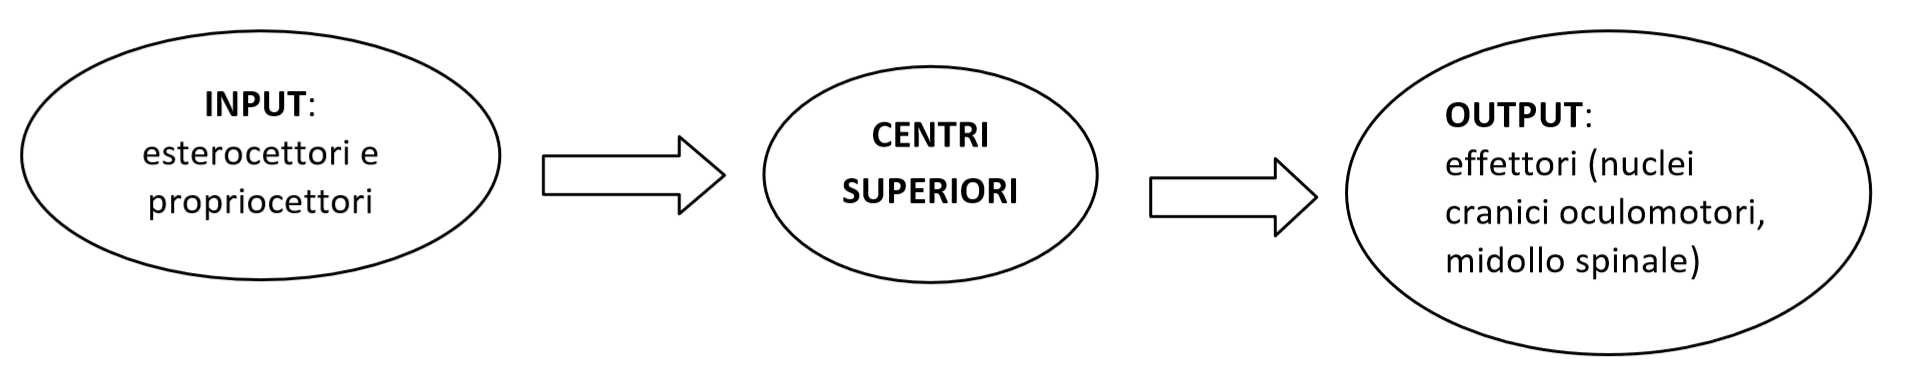
\includegraphics[scale=0.4]{source/immagini/STP.png}
	\caption[Muscoli estrinseci dell'occhio]{Schema del STP, passaggi dell'elaborazione dell'informazione.}
	\label{fig:issuexample}
\end{figure}

\\\ \\\ \\\
\section{L'apparato stomatognatico}

Il complesso stomatognatico svolge funzioni come la masticazione, la deglutizione, la fonazione, la digestione e la respirazione. Esso è formato da:
\begin{itemize}
 \itemsep-0.5em 
 \item[--]una struttura ossea costituita dalle ossa mascellari e palatine, dalla mandibola, dall’articolazione temporo-mandibolare (ATM) e dalle arcate dentarie.
 \item[--]da una struttura miofasciale, costituita  dai muscoli masticatori e dai muscoli di contrappoggio della masticazione (trapezio, sternocleidomastoideo, sopra e sotto-ioidei)
 \item[--]strutture legamentose
 \item[--]innervazione sensitivo-motoria e neuro-vegetativa
 \item[--]organo della lingua.
 \end{itemize}
 
L’organo della lingua (Figura 2.2) merita un approfondimento, poiché fornisce numerose informazioni posturali. Esso è costituito da una porzione anteriore (corpo) ed una posteriore (base), e dal frenulo linguale che collega la superficie ventrale della lingua con il pavimento del cavo orale, in corrispondenza della linea mediana. Nel corpo linguale si distingue l’apice (punta), una faccia superiore (dorso), una inferiore e due bordi laterali. I muscoli estrinseci (Figura 2.3) presenti nella lingua sono: genioglosso (protusore), ioglosso (abbassatore, retrattore), stiloglosso (elevatore e retrattore), palatoglosso (elevatore del corpo), faringoglosso e condroglosso. I muscoli intrinseci sono composti da sistemi di fascetti muscolari detti longitudinali superiore e inferiore, trasversale e verticale. I muscoli intrinseci regolano la forma, mentre gli estrinseci determinano la posizione. 

L’innervazione motoria della lingua è data dal nervo ipoglosso, mentre quella sensitiva dal ramo linguale del nervo trigemino per i due terzi anteriori, dal glossofaringeo per la base e dal nervo laringeo superiore del nervo vago per la zona glossoepiglottica. 

La lingua è coinvolta nelle attività di masticazione, deglutizione e fonazione. Vi sono dei recettori che permettono di controllare la postura della lingua, questi sono: corpuscoli di Meckel, di Pacini, di Meissner, di Ruffini e i propriocettori. La capacità di riconoscere la posizione della lingua e delle strutture anatomiche circostanti, dipende dalle afferenze sensoriali.

\begin{figure}[h!]- 
\centering
\begin{minipage}{.36\textwidth}
  \centering
  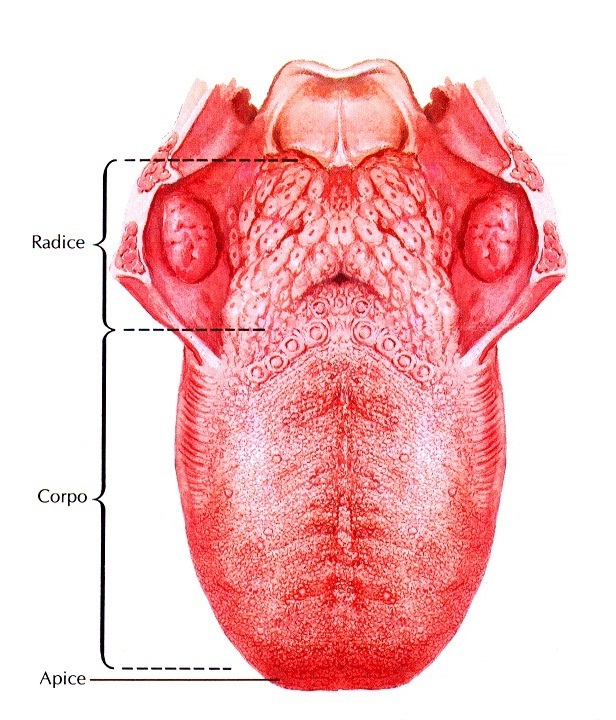
\includegraphics[scale=0.30]{source/immagini/lingua_anatomia.jpg}
  \captionof{figure}{Struttura della lingua.}
  \label{fig:test1}
\end{minipage}%
\begin{minipage}{.5\textwidth}
  \centering
  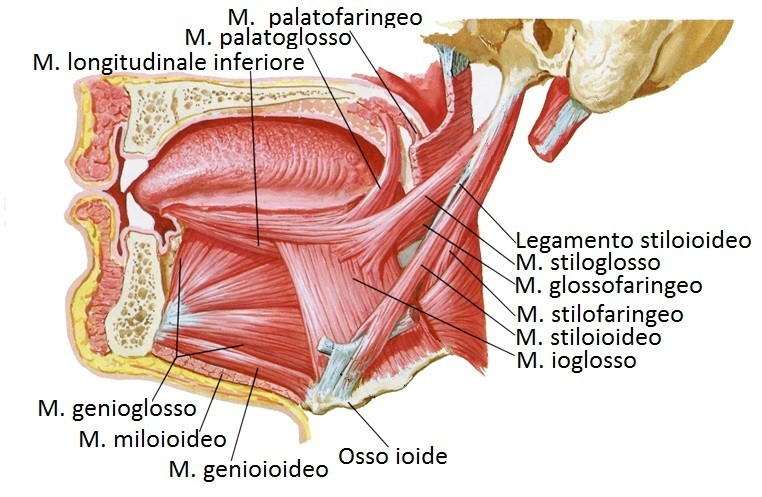
\includegraphics[scale=0.33]{source/immagini/muscoli_estrinseci_lingua.jpg}
  \captionof{figure}{Muscoli estrinseci della lingua.}
  \label{fig:test2}
\end{minipage}
\end{figure}
\\\ \\\ \\\ \\\
Dagli studi di Ferrante\footnote{Dott. Antonio Ferrante: L'importanza della deglutizione nell'ambito gnatologico e posturale (www.ortodonzia.net/deglutizione)}, emerge che, in condizioni fisiologiche, la lingua a riposo deve essere posizionata con l'apice a contatto del palato, subito dietro la papilla retroincisiva, punto corrispondente allo spot linguale, ossia all'emergenza della seconda branca trigeminale dal foro naso-palatino.  Lo spot è situato precisamente tra la papilla interdentale, che si trova nella parte mediana del palato duro, subito dietro gli incisivi superiori, e la prima ruga palatina (Figura 2.4). Di fondamentale importanza per la definizione dello spot e del suo ruolo, sono gli studi di Halata e Baumann (1999)\footnote{Halata Z e Baumann KI, Sensory nerve endings in the hard palate and papilla incisiva of the rhesus monkey, ANAT
EMBRYO, 199(5), 1999, pp. 427-437}, in cui venne indagata l'innervazione sensitiva del palato duro nel macaco Rhesus, dimostrando che nel punto comunemente chiamato spot palatino è presente una quantità elevatissima di cinque diversi esterocettori. 

La postura linguale e la compressione dello spot ad ogni atto deglutitorio comportano la stimolazione dei recettori naso-palatini che continuano ad informare il quinto paio dei nervi cranici. La stimolazione dello spot risulta, quindi, di fondamentale importanza anche durante la funzione deglutitoria. Durante la fase orale della deglutizione i denti vengono a contatto tra loro (massima intercuspidazione) grazie ai muscoli masseteri e temporali, la lingua prende progressivamente contatto con il palato duro a partire dallo spot con movimento antero-posteriore. Il contatto in massima intercuspidazione tra le arcate dentarie durante la fase deglutitoria appena descritta risulta di notevole importanza, perché ciò permette di conferire grande stabilità alla mandibola e, di conseguenza, la lingua avrà la possibilità di compiere un movimento identico e ripetibile, permettendo alla deglutizione di generare un input meccanico e neurologico sempre uguale.

 \begin{figure}[h!]
	\centering
	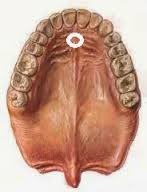
\includegraphics[scale=0.4]{source/immagini/spot_palatino.jpg}
	\caption[Lo spot palatino]{Lo spot palatino.}
	\label{fig:issuexample}
\end{figure}

Tutti gli elementi elencati precedentemente condizionano l’occlusione, cioè il rapporto tra denti superiori e inferiori, i quali dovrebbero cooperare perfettamente. Ciò non avviene quando vi sono delle disfunzioni derivanti da traumi diretti o a distanza che possono creare condizioni che disturbano l’equilibrio della struttura e della funzione stomatognatica con ripercussione neuro-muscolare locale o posturale. L’apparato stomatognatico è anche un recettore posturale, cioè un organo che invia le informazioni al cervello su come interpretare lo spazio. 

Numerose ricerche cliniche dimostrano come un disturbo dell’equilibrio occlusale si ripercuota verso l’insieme del sistema posturale, e viceversa. 
L’apparato stomatognatico presenta infatti molti recettori:
\begin{itemize}
 \itemsep-0.5em 
 \item[--]meccanocettori capsulari, presenti soprattutto nella zona posteriore della capsula. La loro scarica al sistema nervoso centrale permette l’attivazione dei muscoli della mandibola che ne riadattano la postura in base all’informazione inviata. Con il tempo, questo meccanismo cronico provocherà disfunzioni che coinvolgono muscoli di contro-appoggio come trapezio e sternocleidomastoideo, i quali funzionano in sinergia con l’occhio.
 \item[--]recettori muscolari
 \item[--]recettori dentali che sono in grado di rispondere a stimoli infinitesimali. In caso di disfunzione patologica le risposte del sistema nervoso centrale coinvolgono non solo i muscoli dell’apparato stomatognatico, ma anche la muscolatura degli altri distretti come lingua, testa, colonna cervicale.
\end{itemize}
 
\\\ \\\
\section{Influenza dell’occhio e dell’apparato stomatognatico sulla postura}
 
Disfunzioni all’apparato stomatognatico o al sistema visivo possono creare perturbazioni al sistema posturale, costringendolo a riadattarsi. 

La struttura dell’occhio è deputata alla conversione dell’immagine. La possibilità di correzione è relativa, abbastanza limitata e dipende dalle possibilità adattative di messa a fuoco. Questa funzione dipende da: forma dell’occhio, elasticità e trasparenza del cristallino. Riguardo la funzione oculomotoria, l’occhio, grazie alla muscolatura estrinseca, può essere allungato, stirato e compresso da un’alterata azione di questi muscoli. A causa di questi cambiamenti possono verificarsi difetti nella convergenza o alterazioni nella sovrapposizione delle immagini. Quindi fra le disfunzioni oculari che possono intervenire nel determinare uno squilibrio tonico posturale si riconoscono: disturbi di rifrazione, disturbi di convergenza  ed eteroforie. In particolare i disturbi di convergenza e del parallelismo determinano delle necessità di integrazione dello schema corporeo, il quale dovrà scegliere uno schema alternativo a quello ottimale. Il fatto di avere un’eccellente visione non esclude che possa esservi il difetto di convergenza o parallelismo.

La relazione tra sistema visivo e postura nasce dalla prima volta che il bambino solleva la testa e comincia ad osservare ciò che lo circonda. Il perfezionamento del sistema visivo porta al raddrizzamento della posizione della testa, abituandola ad una posizione verticale. Successivamente il sistema vestibolare comincia a migliorare la coordinazione e lo spostamento del capo in diverse posizioni. Questo porta all’acquisizione di diverse esperienze visive le quali vengono integrate con gli altri sistemi. In seguito il sistema visivo ambientale continua ad orientare il corpo nello spazio mentre il sistema visivo focale sviluppa le capacità necessarie per organizzare forme complesse, che saranno necessarie per la lettura. Movimenti oculari ottimali dipendono dalla stabilità del collo, del tronco e dalla mobilità della testa che permettono di trovare il centro di gravità per muoversi nello spazio. Perciò se dovessero verificarsi delle alterazioni delle funzioni visive, il corpo si adatterebbe di conseguenza alle nuove informazioni che riceve, assumendo una postura alterata.
\\\

L’apparato stomatognatico, come precedentemente descritto, è caratterizzato da diverse strutture che agiscono in armonia per svolgere differenti funzioni (parlare, masticare, deglutire). In particolare l’articolazione temporomandibolare (ATM) contrae connessioni muscolari e lagamentose con la regione cervicale, creando un complesso funzionale chiamato sistema cranio-cervico-mandibolare. Il sistema stomatognatico è connesso alla postura grazie all’esistenza delle catene muscolo-fasciali. La fascia è il tessuto connettivo fibroso che, organizzato in foglietti e setti, separa ed unisce ogni parte del corpo. Essa presenta anche una contrattilità autonoma che influenza la postura dell’intero corpo a causa del pretensionamento della catena miofasciale. La catena miofasciale è un gruppo di muscoli interconnessi attraverso la fascia. La sua esistenza può spiegare perchè disordini di funzioni muscolari come masticazione e deglutizione possono essere trasmesse a distanza nel corpo umano. Sempre per questo alterazioni funzionali di una parte del corpo possono creare disordini in un’altra. 

Oltre alla catena miofasciale esiste una via detta oculocefalogira, costituita dalle connessioni neurologiche tra i sistemi. Infatti sono presenti numerose connessioni anatomiche tra i sistemi connessi al trigemino (sistemi trigeminali) e le strutture nervose coinvolte nel mantenimento della postura. I nuclei mesencefalici del trigemino, come visto nel capitolo 1, connettono i neuroni anche esternamente al sistema nervoso centrale e quindi questo spiega il motivo per cui i soggetti con disfunzioni stomatognatiche presentano stimoli in diversi distretti del corpo. Inoltre studi rivelano che esistono connessioni tra il nucleo principale del trigemino e il nucleo vestibolare e preposito dell’ipoglosso. Quest’ultimo è anche un importante centro nervoso per il controllo della posizione e movimento degli occhi, dovuto alla sua stretta relazione con il nucleo vestibolare, il cervelletto e il nucleo oculomotore.
\\\
Altri studi dimostrano la relazione tra l’occlusione dentale, il sistema oculomotore e la stabilità visiva. Monaco ed al. hanno rilevato una maggiore presenza di difetti di convergenza sia in soggetti adulti che presentavano una disfunzione temporo-mandibolare, con dolore miofasciale e all’area del collo e della spalla che in bambini con deviazioni mandibolari laterali. È stato affermato che vi era una maggiore alterazione della funzione binoculare nei soggetti che presentavano queste disfunzioni, piuttosto che nei soggetti sani.  
\\\

Tutte queste connessioni anatomiche suggeriscono che questa porzione di sistemi trigeminali influenza fortemente la coordinazione, la postura e la vista. Sembra che le informazioni sensoriali ricevute dai recettori del sistema stomatognatico vengano integrate con le informazioni  provenienti dai sistemi vestibolare e oculomotore. Le modifiche delle stimolazioni trigeminali possono quindi causare uno sbilanciamento dei sistemi vestibolare ed oculomotore.


\subsection{Ripercussioni dello SMOF sul sistema visivo}
 
Definiamo lo Squilibrio Muscolare Oro-Facciale (SMOF) come un’alterazione dell’equilibrio delle strutture del complesso bucco-facciale, quindi dell’apparato stomatognatico, che può essere causata da:

\begin{itemize}
 \itemsep-0.5em 
 \item[--]mancato passaggio dalla deglutizione infantile a quella adulta con la corretta postura linguale e quindi corretta deglutizione
 \item[--]malocclusioni dentali
 \item[--]respirazione orale, a causa di patologie o di allergie
 \item[--]scorretta postura della lingua determinata da vizi orali (succhiamento del pollice, prolungato uso del ciuccio o biberon..)
 \item[--]traumi o ferite al complesso oro-facciale
 \item[--]disfunzioni del sistema nervoso centrale
\end{itemize}
Le conseguenze dello SMOF e in particolare della funzione deglutitoria si ripercuotono sia sulla postura che su altri distretti corporei. La deglutizione, attraverso la stimolazione trigeminale, può interferire con i recettori posturali principali, tra cui l’occhio. Il motivo per cui i recettori occhio e bocca si influenzano reciprocamente è descritto dalla via \emph{oculocefalogira}. Essa è costituita da:
\begin{itemize}
 \itemsep-0.5em 
 \item[--]una via ascendente, che trasporta le informazioni propriocettive dai recettori paradontali delle arcate superiori e dai recettori dello spot palatino al nucleo mesencefalico del trigemino e da qui proietta ai nuclei del III, IV, VI nervo cranico
 \item[--]una via discendente, dove le afferenze provenienti dall’apparato stomatognatico, proiettano le informazioni al nucleo mesencefalico del trigemino, il quale comunica con il nucleo accessorio spinale, nelle corna anteriori del midollo cervicale (C1-C5). Da qui parte il nervo accessorio (XI) che innerva il muscolo trapezio superiore e lo SCOM (sterno-cleido-occipito-mastideo). Inoltre dai muscoli oculomotori partono fibre che arrivano ai nuclei oculomotori e poi raggiungono il nucleo del trigemino, il quale è coinvolto anche nell’apertura e chiusura della mandibola e nella masticazione.
\end{itemize}
\\\
Un disturbo visivo (foria, insufficienza accomodativa, ipoconvergenza, ecc..) può influenzare l’occlusione dentale attraverso variazioni della posizione della testa mediate dal sistema oculocefalogiro ed atte al compenso funzionale del difetto. Però è vero anche che una malocclusione o una deglutizione atipica può determinare una posizione viziata della testa, quindi il sistema visivo dovrebbe adattarsi alla nuova posizione e modificherebbe il suoi parametri. Quindi sebbene l’apparato stomatognatico e il sistema visivo siano funzionalmente distinti, esiste una correlazione sia a livello neurofisiologico, per la comunicazione dei nervi trigemino, oculomotore e accessorio (via oculocefalogira), sia a livello neuromuscolare, per le catene muscolo-connettivali (catene miofasciali).
